\chapter{Befehle, Gruppen, Umgebungen und Zeichen}
\label{BefehleGruppenUmgebungenZeichenKapitel}

In diesem Kapitel erfahren Sie, was in der Auszeichnungssprache von \LaTeX\ Befehle und Umgebungen sind, und wie Sie mit diesen arbeiten können. Zudem enthält dieses Kapitel einige wichtige Sonderzeichen und präsentiert eine Auswahl grundlegender Befehle und Umgebungen anhand von Beispielen.

\section{Befehle}
\index{Befehle}

Wie auf Seite~\pageref{Seite_Befehl} beschrieben, leitet der Backslash (\verb!\!), der sogenannte \emph{Escape Character} LaTeX-Befehle ein. Befehle können mehrere Argumente haben. Zwingende Argumente\index{Argument!zwingend} stehen meist in geschweiften\index{Klammern!geschweift} Klammern \verb!{...}!, in manchen Fällen
auch in runden\index{Klammern!rund} \verb!(...)!. Optionale Argumente sind in eckigen\index{Klammern!eckig} Klammern \verb![...]! angegeben.

\fbox{\texttt{\textbackslash}\textsl{befehl}\texttt{[}\textsl{optionale Argumente}\texttt{]}\texttt{\{}\textsl{zwingende Argumente}\texttt{\}}}

In den allermeisten Fällen Befehle mit Kleinbuchstaben geschrieben. Dabei ist zu beachten, dass \LaTeX\ \emph{case sensitive} arbeitet. Es unterscheidet also bei den Namen von Befehlen zwischen Groß- und Kleinschreibung. Zudem dürfen die Namen von Befehlen nur Buchstaben enthalten. 

Jede Zeile kann mehrere Befehle enthalten und die Reichweite eines Befehls beginnt ab der Stelle im Quelltext, wo er auftritt, bis zum Ende der lokalen Gruppe.


\section{Gruppen}
\index{Gruppe}

Eine Gruppe ist ein Textbereich, der von geschweiften Klammern eingeschlossen ist. Der Inhalt 
einer Gruppe beginnt also nach \verb!{! und reicht bis zur nächsten  schließenden geschweiften Klammer \verb!}!.

Gruppen werden häufig verwendet, um einen Textabschnitt in einer anderen Schriftart oder Schriftgröße zu setzen. Dafür wird vor den Text der Gruppe der gewünschte Befehl geschrieben. Dieser Befehl hat dann auch nur innerhalb der geschweiften Klammern Gültigkeit. Einige Beispiele für Gruppen enthält Listing~\ref{zweitesbeispiel}. Das Ergebnis dieses Beispiels zeigt Abbildung~\ref{fig_Listing2}.

\lstinputlisting[caption={Ein Beispiel zu Gruppen},label=zweitesbeispiel, style=customlatex]{Beispiele/Gruppen/gruppen.tex}

\begin{figure}[H]
%     \centering
         % Abschneiden mit trim = liks unten rechts oben
         \fbox{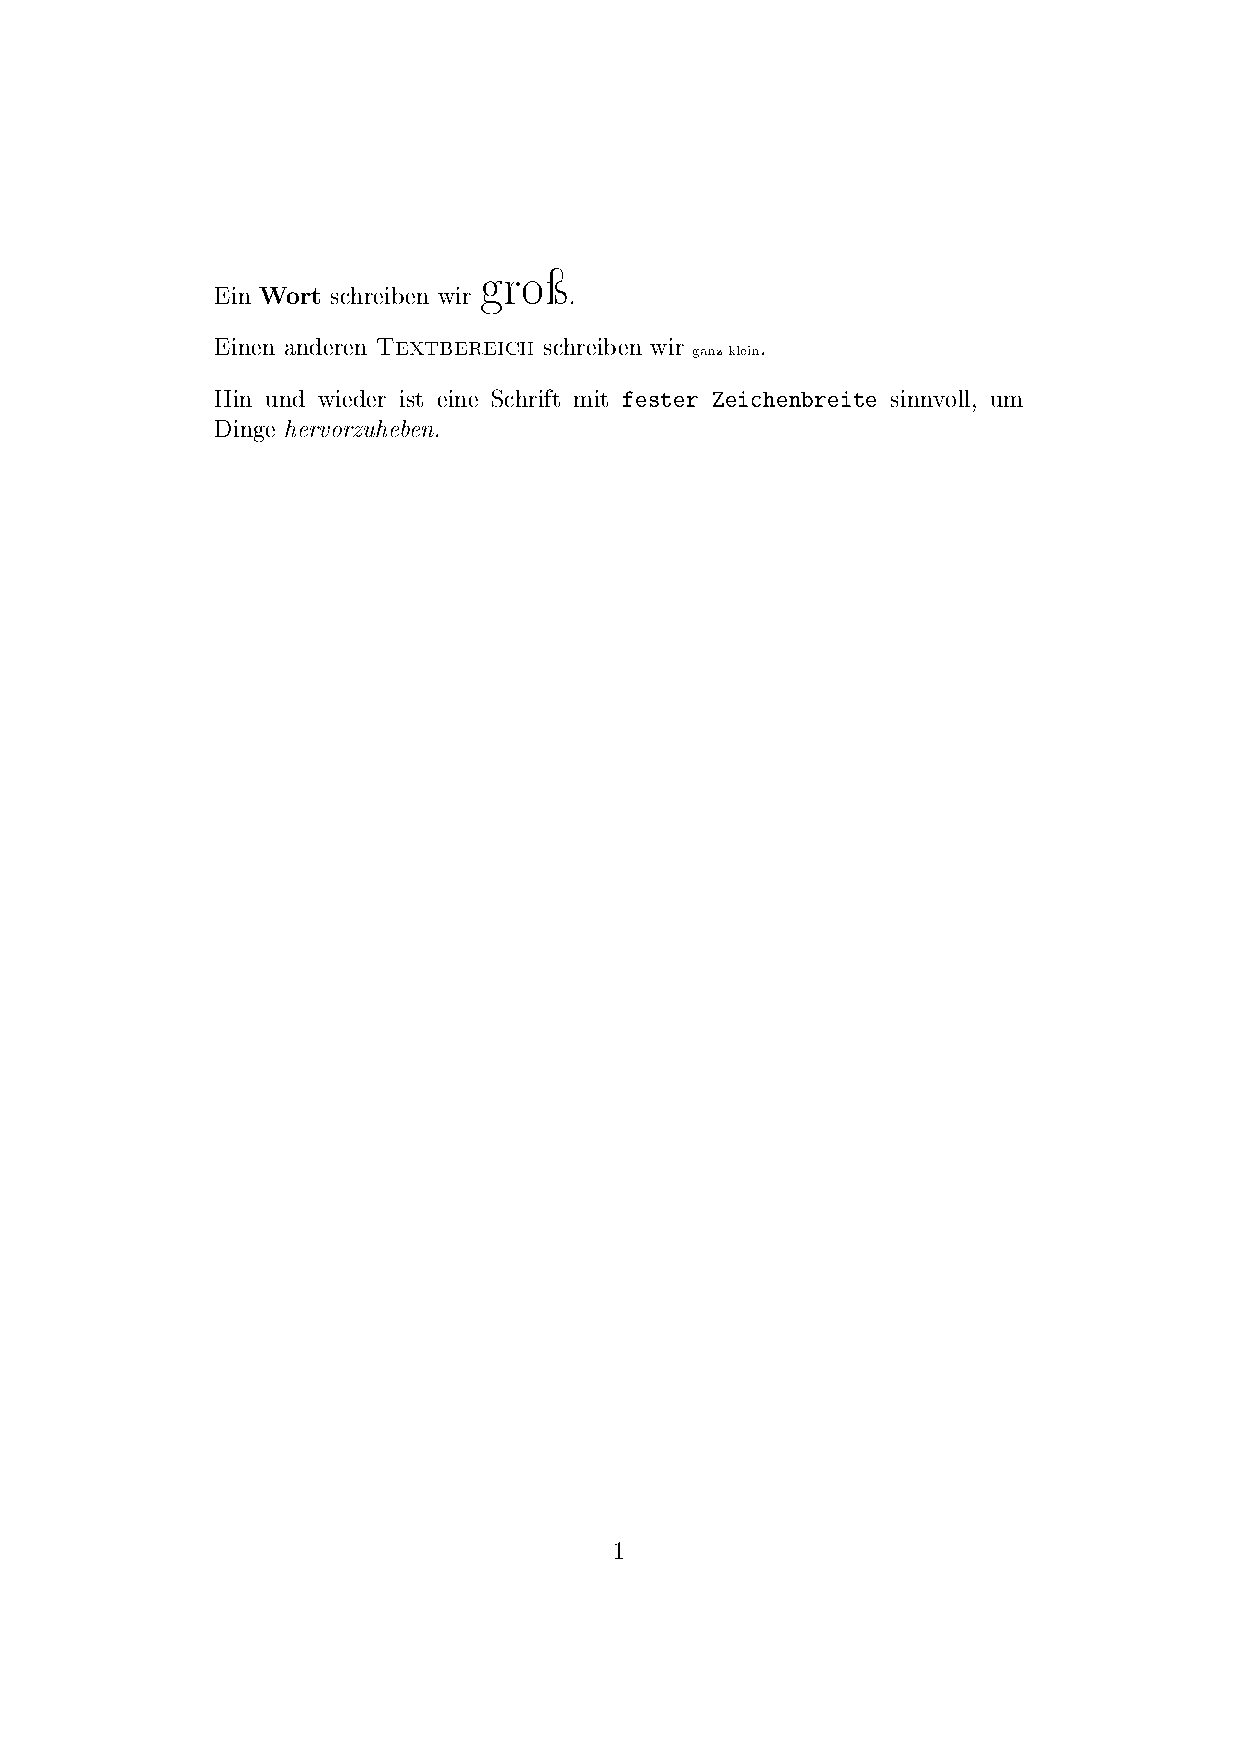
\includegraphics[page=1, clip, trim=3cm 21.5cm 3cm 4cm, width=.98\textwidth]{Beispiele/Gruppen/gruppen.pdf}}
    \caption{Resultat von Listing~\ref{zweitesbeispiel}}
    \label{fig_Listing2}
\end{figure}


\section{Umgebungen}
\index{Umgebung}

Umgebungen beginnen mit dem Befehl \verb!\begin{!\textsl{Umgebung}\verb!}!
und enden mit dem Befehl \verb!\end{!\textsl{Umgebung}\verb!}!.

Zwischen dem Anfang und dem Ende einer Umgebung können Texte und auch
Befehle stehen. Allerdings sind nicht alle Befehle innerhalb aller
Umgebungen zulässig. Ein Beispiel dafür ist der Befehl \verb!\verb! zum
Satz unformatierter Texte mit fester Zeichenbreite. Dessen Verwendung ist bei zahlreichen Umgebungen nicht zulässig.

Es ist auch möglich, Umgebungen miteinander zu verschalten. Das ist beispielsweise nötig, um Aufzählungen mit mehreren Ebenen (siehe Abschnitt~\ref{Abschnitt_Aufzaehlungen}) zu realisieren.



\section{Maßangaben mit absoluten und relativen Maßeinheiten}
\index{Massangaben}
\index{Maßeinheit}

Maßeinheiten und feste\index{Maßeinheit!fest} sowie elastische\index{Maßeinheit!fest} Maße ermöglichen es, das Layout von Dokumenten zu definieren. 

Maßangaben bestehen aus mindestens einer Dezimalzahl\index{Dezimalzahl} (mit oder ohne Vorzeichen) und aus einer 
Maßeinheit, die direkt (ohne Leerzeichen) auf die Zahl folgt. Eine Übersicht über die unterstützten Maßeinheiten zeigt Tabelle~\ref{Tabelle_Masseinheiten}. Dezimalzahlen dürfen bei \LaTeX\ mit einem Komma oder alternativ mit einem Dezimalpunkt\index{Dezimalpunkt} geschrieben werden, um die Nachkommastellen kenntlich zu machen. Somit sind beispielsweise \verb!3.5cm! und 
\verb!3,5cm!, sowie \verb!3cm! erlaubte Angaben.

\LaTeX\ kennt neun absolute und zwei relative Maßeinheiten. Die relativen Maßeinheiten \verb!em! und \verb!ex! orientieren sich an der aktuell verwendeten Schriftart. 



\begin{table}[h!tb]
\centering
\caption[Absolute und relative Maßeinheiten]{Absolute und relative Maßeinheiten~\cite{Schwarz1988}}
\label{Tabelle_Masseinheiten}       % Give a unique label
\begin{tabular}{clll}
\hline
Abkürzung & Bedeutung & \multicolumn{2}{c}{Umrechnungen}  \\
\hline
\texttt{pt} & \glqq\textsl{Point}\grqq\ (Punkt) & 1\,pt = 0,013837\,in & 1\,pt = 0,0351\,cm \\
\texttt{pc} & Pica & 1\,pc = 12\,pt & 1\,pc = 0,422\,cm \\
\texttt{in} & \glqq\textsl{Inch}\grqq\ (Zoll) & 1\,in = 72,27\,pt & 1\,in = 2.54\,cm \\
\texttt{mm} & Millimeter & 1\,mm = 2,845\,pt \\
\texttt{cm} & Zentimeter & 1\,cm = 28,45\,pt & 1\,cm = 10\,mm\\
\texttt{bp} & Big Point & 72\,bp = 1\,in & 1\,bp = 0,03528\,cm\\
\texttt{dd} & Didot Punkt & 1157\,dd = 1238\,pt & 1\,dd = 0,03761\,cm\\
\texttt{cc} & Cicero & 1\,cc = 12\,dd & 1\,cc = 0,45132\,cm \\
\texttt{sp} & Scaled Point & 65536\,sp = 1\,pt & 1\,sp \(<\) 0,6 \(*\) 10\textsuperscript{-6}\,cm\\
\texttt{em} & Geviert & \multicolumn{2}{l}{Relatives Maß. Ist ca. die Breite von \glqq M\grqq} \\  
\texttt{ex} & & \multicolumn{2}{l}{Relatives Maß. Ist ca. die Höhe von \glqq x\grqq} \\ 
\hline
\end{tabular}
\end{table}
% Solche Tabellen/Gegenüberstellungen finden sich in allen Dokumentationen zu TeX/LaTeX


Das \emph{Geviert}\index{Geviert} und ist eine typografische Maßeinheit 
aus der Zeit des Bleisatzes mit beweglichen Lettern. Ein Geviert bezeichnet dabei die Schriftgröße (Kegelhöhe)\index{Kegelhöhe}. Bei einer Schriftgröße von 12\,Punkten hat ein Geviert dementsprechend eine Länge von 12\,Punkten~\cite{LeerraumGevierte_Webpage}. 

Bei der Arbeit mit \LaTeX\ kommt es häufig vor, dass Absatzeinzüge\index{Absatzeinzüge} 
in Geviert angegeben sind (meist \verb!1em! oder \verb!2em!). Auch die konkreten Längen der unterschiedlichen horizontalen Striche im Text -- Geviertstrich\index{Geviertstrich}, Halbgeviertstrich\index{Halbgeviertstrich} (Gedankenstrich)\index{Gedankenstrich} und Viertelgeviertstrich\index{Viertelgeviertstrich} (Bindestrich)\index{Bindestrich} hängen von der Seitenlänge des Gevierts und damit von der Schriftgröße ab~\cite{Geviert_Wiki_Webpage}.

Während das relative Maß \verb!em! meist für horizontalen Maße verwendet\index{Maß!horizontal} wird, eignet sich \verb!ex! besonders für vertikale Maße\index{Maß!vertikal}. 

In der Literatur zu \LaTeX\ findet sich auch immer wieder die Aussage, dass \verb!em! etwas der 
Breite des Großbuchstabens \glqq M\grqq\ und \verb!ex! in etwa der Höhe des Buchstabens \glqq x\grqq\ im aktuellen Font entspricht.~\cite{Kopka2000,Schwarz1988}


% Quellen: Schwarz1988: S.22
% Kopka2000: S.14


\subsection{Anwendungsbeispiele}

Mit den in diesem Abschnitt beschriebenen Maßeinheiten werden unter anderem 
Längenbefehlen\index{Längenbefehle}, die das Dokumentenlayout definieren, Werte zugewiesen

Um beispielsweise die Höhe und Breite des Textes festzulegen, müssen den Längenbefehlen \verb!\textheight! und \verb!\textwidth! mit dem Befehl \verb!\setlength! die gewünschten Werte zugewiesen werden.


\fbox{\texttt{\textbackslash setlength\{\textbackslash \textsl{Längenbefehl}\}\{\textsl{Maßangabe}\}}}


Soll beispielsweise ein Dokument eine Texthöhe\index{Texthöhe} von 18\,cm und eine
Textbreite\index{Textbreite} von 13,5\,cm haben, muss dieses mit den folgenden beiden Zeilen in der Präambel der \verb!.tex!-Quelldatei definiert werden.


\begin{Verbatim}[frame=single]
\setlength{\textwidth}{13.5cm}
\setlength{\textheight}{18cm}
\end{Verbatim}

Weitere häufige Anwendungsbeispiele, wo die Maßangaben eine Rolle spielen, sind Befehle um horizontale oder vertikale Abstände zu definieren, wie zum Beispiel \verb!\hspace! und \verb!\vspace!, sowie Abbildungen und Tabellen.

\subsection{Elastische Maße}
\label{Elastische_Masse}

Der Unterschied zwischen festen und elastischen 
Maßen ist, das elastische Maße um festzulegende Werte gestreckt und gestaucht werden
können. Die Definition eines elastischen Maßes erfolgt mit drei Werten~\cite{Kopka2000}: 

\begin{itemize}
\item Sollwert 
\item Streckwert -- der Wert, um den maximal gestreckt werden darf
\item Stauchwert -- der Wert, um den maximal gestaucht werden darf
\end{itemize}

Die Syntax für ein elastisches Maß ist:


\fbox{\texttt{\textbackslash setlength\{\textbackslash \textsl{Befehl}\}\{\textsl{Sollwert} plus \textsl{Streckwert} minus \textsl{Stauchwert}\}}}

Das folgende Beispiel zeigt ein Anwendungsbeispiel. Dieses definiert den Zeilenabstand zwischen Absätzen auf elastische Art und Weise.

\begin{Verbatim}[frame=single]
\setlength{\parskip}{2ex plus 0.3ex minus 0.5ex}
\end{Verbatim}

Konkret ist hier definiert, das der Abstand zwischen zwei 
Absätzen zweimal so hoch sein soll, wie der Buchstabe \glqq x\grqq\ im aktuellen Zeichensatz hoch ist. Der Abstand darf bei Bedarf bis auf den 2,3-fachen Abstand gedehnt oder auf den 1,5-fachen Abstand gestaucht werden.


\section{Sonderzeichen}

Sonderzeichen sind unter \LaTeX\ einerseits
Zeichen, die eine besondere Funktion haben (beispielsweise \verb!&! und
\verb!$!), andererseits sind Sonderzeichen aber auch Zeichen, für die auf 
einer normalen Tastatur keine Taste existiert (zum Beispiel
\copyright, \dag und \ddag).

Buchstaben mit Akzenten sind im Grunde auch so etwas wie 
Sonderzeichen und Anführungszeichen\index{Anführungszeichen} 
aller Art sowie Punkte und Striche
der verschiedensten Form kann man auch als Sonderzeichen bezeichnen.


\subsection{Besondere Zeichen}

\LaTeX\ kennt eine große Zahl besonderer Zeichen, die auch Sonderzeichen heißen. Dieser Abschnitt präsentiert eine Auswahl an vergleichsweise häufig verwendeten besonderen Zeichen. Diese sind:


\begin{center}
\textbackslash\ \quad \$ \quad \& \quad \% \quad \# \quad \_  
\quad \textasciitilde\ \quad \textasciicircum\ \quad \{ \quad \}
\end{center}


Diese besonderen Zeichen haben bei der Texteingabe eine spezielle Bedeutung (siehe Tabelle~\ref{Tabelle_Sonderzeichen}) und die meisten von ihnen können durch das Voranstellen eines Backslashs\index{Backslash} (\verb!\!) dargestellt werden.

\begin{table}[h!tb]
\centering
\caption{Besondere Zeichen}
\label{Tabelle_Sonderzeichen}       % Give a unique label
\begin{tabular}{cp{6.7cm}p{4cm}}
\hline
Zeichen & Bedeutung des Zeichens & Befehl \\
\hline
\textbackslash & Mit einem Backslash beginnt ein Befehl  & \texttt{\textbackslash textbackslash} \\
\$ & Schaltet in den Mathematikmodus um & \texttt{\textbackslash \$} \\
\& & Markiert die Grenzen der Tabellenspalten & \texttt{\textbackslash \&} \\
\% & Alles bis zum Zeilenende wird ignoriert & \texttt{\textbackslash \%} \\
\# & Makroparameterzeichen & \texttt{\textbackslash \#} \\ 
\_ & Definiert im Mathematikmodus Indizes & \texttt{\textbackslash textunderscore} oder \texttt{\textbackslash \_} \\
\textasciitilde & Fügt einen untrennbaren Zwischenraum ein & \texttt{\textbackslash textasciitilde} \\
\textasciicircum & Definiert im Mathematikmodus Exponenten 
 & \texttt{\textbackslash textasciicircum} \\
\{ & Definiert den Anfang einer Gruppe & \texttt{\textbackslash\{} \\
\} & Definiert das Ende einer Gruppe &  \texttt{\textbackslash\}} \\
\hline
\end{tabular}
\end{table}



\subsection{Einige häufig verwendete Zeichen bzw. Symbole}

\LaTeX\ bietet eine große Anzahl von Zeichen, die auch Symbole heißen. Tabelle~\ref{Tabelle_Symbole} präsentiert einige der häufiger verwendeten.


\begin{table}[h!tb]
\centering
\caption{Zeichen (Symbole)}
\label{Tabelle_Symbole}       % Give a unique label
\begin{tabular}{cll}
\hline
Symbol & Bezeichnung & Schreibweise \\ 
\hline
\copyright & Copyright\index{Copyright} & \texttt{\textbackslash copyright} \\
\textregistered & Registered\index{Registered-Zeichen} & \texttt{\textbackslash textregistered} \\
\texttrademark & Trademark\index{Trademark-Zeichen} & \texttt{\textbackslash texttrademark} \\
\S & Juristischer Paragraph & \texttt{\textbackslash S}\\
\P & Paragraph\index{Paragraph-Zeichen} & \texttt{\textbackslash P}\\
\euro & Euro\index{Euro} & \texttt{\textbackslash euro} \\
\pounds & Pfund Sterling\index{Pfund Sterling} & \texttt{\textbackslash pounds} \\
\textyen & Yen\index{Yen} & \texttt{\textbackslash textyen} \\
\dag & Dagger\index{Dagger-Zeichen} & \texttt{\textbackslash dag} \\
\ddag & Doppel-Dagger\index{Doppel-Dagger-Zeichen} & \texttt{\textbackslash ddag} \\ 
\textbullet & Aufzählungspunkt\index{Aufzählungspunkt} & \texttt{\textbackslash textbullet} \\
@ & Klammeraffe & \texttt{@} \\
\hline
\end{tabular}
\end{table}

Auch für die in diesem Dokument schon mehrfach verwendeten Schriftzüge von \TeX\ und \LaTeX\ gibt es entsprechende Befehle. Diese enthält Tabelle~\ref{Tabelle_Schriftzuege}.

\begin{table}[h!tb]
\centering
\caption{Befehle zum komfortablen Satz der \TeX/\LaTeX-Schriftzüge}
\label{Tabelle_Schriftzuege}       % Give a unique label
\begin{tabular}{cll}
\hline
Symbol & Bezeichnung & Befehl \\ 
\hline
\TeX & Schriftzug von \TeX & \texttt{\textbackslash TeX} \\
\LaTeX & Schriftzug von \LaTeX & \texttt{\textbackslash LaTeX} \\
\LaTeXe & Schriftzug der seit 1994 aktuellen Version von \LaTeX & \texttt{\textbackslash LaTeXe} \\
\hline
\end{tabular}
\end{table}


Eine sehr große Zahl weiter Zeichen enthält das Erweiterungspaket \verb!textcomp.sty!, das mit dem Befehl \verb!\usepackage{textcomp}! in der Präambel eines \LaTeX-Quelltextes eingebunden. Eine Auswahl der Befehle im Paket \verb!textcomp! enthält Tabelle~\ref{Tabelle_SymboleTextcomp}.



% \begin{table}[h!tb]
% \centering
\begin{longtable}{lclc}
\caption{Zeichen aus dem Erweiterungspaket \texttt{textcomp}}
\label{Tabelle_SymboleTextcomp}       % Give a unique label
\endfirsthead
\endhead
\hline
Befehl  & Zeichen &  Befehl & Zeichen  \\  
\hline
\texttt{\textbackslash textdollaroldstyle} & \textdollaroldstyle &
\texttt{\textbackslash textcentoldstyle} & \textcentoldstyle \\
\texttt{\textbackslash textdollar} & \textdollar &
\texttt{\textbackslash textcent} & \textcent \\[1em]
\texttt{\textbackslash textzerooldstyle} & \textzerooldstyle &
\texttt{\textbackslash textoneoldstyle} & \textoneoldstyle \\
\texttt{\textbackslash texttwooldstyle} & \texttwooldstyle &
\texttt{\textbackslash textthreeoldstyle} & \textthreeoldstyle \\
\texttt{\textbackslash textfouroldstyle} & \textfouroldstyle &
\texttt{\textbackslash textfiveoldstyle} & \textfiveoldstyle \\
\texttt{\textbackslash textsixoldstyle} & \textsixoldstyle &
\texttt{\textbackslash textsevenoldstyle} & \textsevenoldstyle \\
\texttt{\textbackslash texteightoldstyle} & \texteightoldstyle &
\texttt{\textbackslash textnineoldstyle} & \textnineoldstyle \\[1em]
\texttt{\textbackslash texttimes} & \texttimes &
\texttt{\textbackslash textonesuperior} & \textonesuperior \\
\texttt{\textbackslash texttwosuperior} & \texttwosuperior &
\texttt{\textbackslash textthreesuperior} & \textthreesuperior \\
\texttt{\textbackslash textonequarter} & \textonequarter &
\texttt{\textbackslash textonehalf} & \textonehalf \\
\texttt{\textbackslash textthreequarters} & \textthreequarters &
\texttt{\textbackslash textsurd} & \textsurd \\
\texttt{\textbackslash textperthousand} & \textperthousand & & \\[1em]
\texttt{\textbackslash textrightarrow} & \textrightarrow &
\texttt{\textbackslash textleftarrow} & \textleftarrow \\
\texttt{\textbackslash textuparrow} & \textuparrow &
\texttt{\textbackslash textdownarrow} & \textdownarrow \\[1em]
\texttt{\textbackslash textdagger} & \textdagger &
\texttt{\textbackslash textdaggerdbl} & \textdaggerdbl \\
\texttt{\textbackslash textohm} & \textohm &
\texttt{\textbackslash textmho} & \textmho \\
\texttt{\textbackslash textlbrackdbl} & \textlbrackdbl &
\texttt{\textbackslash textrbrackdbl} & \textrbrackdbl \\[1em]
\texttt{\textbackslash textcopyright} & \textcopyright &
\texttt{\textbackslash textcopyleft} & \textcopyleft \\
\texttt{\textbackslash textregistered} & \textregistered &
\texttt{\textbackslash textcircledP} & \textcircledP \\
\texttt{\textbackslash texttrademark} & \texttrademark &
\texttt{\textbackslash textservicemark} & \textservicemark \\
\texttt{\textbackslash textnumero} & \textnumero &
\texttt{\textbackslash textestimated} & \textestimated \\[1em]
\texttt{\textbackslash textdegree} & \textdegree &
\texttt{\textbackslash textcelsius} & \textcelsius \\
\texttt{\textbackslash textbullet} & \textbullet &
\texttt{\textbackslash textopenbullet} & \textopenbullet \\
\texttt{\textbackslash textasteriskcentered} & \textasteriskcentered &
\texttt{\textbackslash textmusicalnote} & \textmusicalnote \\
\texttt{\textbackslash textordfeminine} & \textordfeminine &
\texttt{\textbackslash textordmasculine} & \textordmasculine\\
\texttt{\textbackslash textlquill} & \textlquill &
\texttt{\textbackslash textrquill} & \textrquill \\
\texttt{\textbackslash textbardbl} & \textbardbl &
\texttt{\textbackslash textbrokenbar} & \textbrokenbar \\[1em]
\texttt{\textbackslash textthreequartersemdash} & \textthreequartersemdash &
\texttt{\textbackslash texttwelveudash} & \texttwelveudash \\
\texttt{\textbackslash texttimes} & \texttimes &
\texttt{\textbackslash textdiv} & \textdiv \\
\texttt{\textbackslash textminus} & \textminus &
\texttt{\textbackslash textdblhyphen} & \textdblhyphen \\
\texttt{\textbackslash textdiscount} & \textdiscount &
\texttt{\textbackslash textfractionsolidus} & \textfractionsolidus \\
\texttt{\textbackslash textlangle} & \textlangle &
\texttt{\textbackslash textrangle} & \textrangle \\[1em]
\texttt{\textbackslash textparagraph} & \textparagraph &
\texttt{\textbackslash textpilcrow} & \textpilcrow \\
\texttt{\textbackslash textreferencemark} & \textreferencemark &
\texttt{\textbackslash textcurrency} & \textcurrency \\
\texttt{\textbackslash textsection} & \textsection &
\texttt{\textbackslash textbigcircle} & \textbigcircle \\[1em]
\texttt{\textbackslash textquotestraightdblbase} & \textquotestraightdblbase &
\texttt{\textbackslash textquotestraightbase} & \textquotestraightbase \\
\texttt{\textbackslash textquotesingle} & \textquotesingle &
\texttt{\textbackslash texttildelow} & \texttildelow \\
\texttt{\textbackslash textasciibreve} & \textasciibreve &
\texttt{\textbackslash textasciicaron} & \textasciicaron \\
\texttt{\textbackslash textperiodcentered} & \textperiodcentered &
\texttt{\textbackslash textasciidieresis} & \textasciidieresis \\
\texttt{\textbackslash textlnot} & \textlnot &
\texttt{\textbackslash textdblhyphenchar} & \textdblhyphenchar \\
\texttt{\textbackslash textpm} & \textpm &
\texttt{\textbackslash textasciimacron} & \textasciimacron \\
\texttt{\textbackslash textgravedbl} & \textgravedbl &
\texttt{\textbackslash textacutedbl} & \textacutedbl \\
\texttt{\textbackslash textasciigrave} & \textasciigrave &
\texttt{\textbackslash textasciiacute} & \textasciiacute \\
\hline
\end{longtable}
% \end{table}


% \par
% \begin{tabularx}{\textwidth}{>{\setlength{\hsize}{1.3\hsize}}X%
% >{\setlength{\hsize}{.7\hsize}}Y>{\setlength{\hsize}{1.3\hsize}}X%
% >{\setlength{\hsize}{.7\hsize}}Y}
% \texttt{\textbackslash textquotestraightdblbase} & \textquotestraightdblbase &
% \texttt{\textbackslash textquotestraigh!tbase} & \textquotestraigh!tbase \\
% \texttt{\textbackslash textquotesingle} & \textquotesingle &
% \texttt{\textbackslash texttildelow} & \texttildelow \\
% \texttt{\textbackslash textasciibreve} & \textasciibreve &
% \texttt{\textbackslash textasciicaron} & \textasciicaron \\
% \texttt{\textbackslash textperiodcentered} & \textperiodcentered &
% \texttt{\textbackslash textasciidieresis} & \textasciidieresis \\
% \texttt{\textbackslash textlnot} & \textlnot &
% \texttt{\textbackslash textdblhyphenchar} & \textdblhyphenchar \\
% \texttt{\textbackslash textpm} & \textpm &
% \texttt{\textbackslash textasciimacron} & \textasciimacron \\
% \texttt{\textbackslash textgravedbl} & \textgravedbl &
% \texttt{\textbackslash textacutedbl} & \textacutedbl \\
% \texttt{\textbackslash textasciigrave} & \textasciigrave &
% \texttt{\textbackslash textasciiacute} & \textasciiacute \\
% \end{tabularx}
% \begin{tabularx}{\textwidth}{Y}
% \rowcolor[gray]{0.9}
% \textsl{Tabelle 5.6: Auswahl an Zeichen aus dem \texttt{textcomp}-Paket}
% \end{tabularx}


\subsection{Punkte und Striche}

Tabelle~\ref{Tabelle_Horizontale_Striche} zeigt eine Übersicht über die Befehle von \LaTeX, um unterschiedliche Arten von horizontalen Strichen zu setzen. 

\begin{table}[h!tb]
	\centering
	\caption{Horizontale Striche}
	\label{Tabelle_Horizontale_Striche}       % Give a unique label
	\begin{tabular}{cll}
		\hline
		Symbol & Bezeichnung & Befehl \\ 
		\hline
		- & Trenn-/Bindestrich & \texttt{-} oder \texttt{\textbackslash texthyphenchar}\\
		-- & Gedankenstrich & \texttt{-{}-} oder \texttt{\textbackslash textendash} \\
		--- & längerer Gedankenstrich & \texttt{-{}-{}-} oder \texttt{\textbackslash textemdash} \\
		\hline
	\end{tabular}
\end{table}

Der Trennstich\index{Trennstich} (-), der auch Viertelgeviertstrich\index{Viertelgeviertstrich} heißt, wird als Trennzeichen beim Trennen von Wörtern, oder als \textsl{Bindestrich}\index{Bindestrich} in zusammengesetzten Begriffen benutzt. Er wird wie ein ganz gewöhnlicher horizontaler Strich (\texttt{-}) geschrieben.

Der Gedankenstrich\index{Gedankenstrich} (--), der auch Halbgeviertstrich\index{Halbgeviertstrich} heißt, wird oft bei Strecken- oder Zeitangaben benutzt. Er wird mit zwei Strichen (\texttt{-{}-}) oder alternativ mit dem Befehl \verb!\textendash! erzeugt.

Primär im englischen Sprachraum wird in Dokumenten ein längerer 
Gedankenstrich (---), der sogenannte Geviertstrich\index{Geviertstrich}, verwendet. Dieser wird mit drei Strichen (\texttt{-{}-{}-}) oder dem Befehl \verb!\textemdash! erzeugt. 

\begin{table}[h!tb]
	\centering
	\caption{Fortsetzungspunkte mit \LaTeX}
	\label{Tabelle_Horizontale_Punkte}       % Give a unique label
	\begin{tabular}{cll}
		\hline
		Symbol & Bezeichnung & Befehl \\ 
		\hline
		. & gewöhnlicher Punkt & \texttt{.} \\
		... & drei gewöhnliche Punkte & \texttt{...} \\
		\dots & Fortsetzungspunkte & \texttt{\textbackslash dots}  \\
		\hline
	\end{tabular}
\end{table}


Auf den ersten Blick erscheint es kurios, das \LaTeX\ mit \verb!\dots! einen Befehl bietet, um drei aufeinander folgende Punkte, so genannte Fortsetzungspunkte\index{Fortsetzungspunkte}, zu setzen. Der Grund, warum dieser Befehl sehr sinnvoll ist, ist der Abstand zwischen den Fortsetzungspunkten. Schreibt ein Autor einfach drei Punkte hintereinander, ist der Abstand zwischen den Punkten recht klein. Der Befehl \verb!\dots! erzeugt ein optisch besseres Ergebnis. Tabelle~\ref{Tabelle_Horizontale_Punkte} zeigt den Unterschied. 



\subsection{Anführungszeichen}

\LaTeX\ ermöglicht den Satz verschiedener Anführungszeichen. Eine Übersicht präsentiert Tabelle~\ref{Tabelle_Anfuehrungszeichen}. 

\begin{table}[h!tb]
\centering
\caption{Anführungszeichen}
\label{Tabelle_Anfuehrungszeichen}       % Give a unique label
\begin{tabular}{lll}
\hline
Anführungszeichen & Kurzform & Befehl \\
\hline
\dq Doublequotes\dq & \texttt{\textbackslash dq} & \texttt{\textbackslash dq} oder \texttt{\textbackslash doublequotedbl} \\
\glqq deutsche Anführungszeichen\grqq & \texttt{\dq `}& \texttt{\textbackslash glqq} oder \texttt{\textbackslash quotedblbase} \\
& \texttt{\dq '} & \texttt{\textbackslash grqq} oder \texttt{\textbackslash quotedbrbase} \\
\glq Halbe deutsche\grq  & & \texttt{\textbackslash glq} oder \texttt{\textbackslash quotedsinglbase}\\
& & \texttt{\textbackslash grq} oder \texttt{\textbackslash quotedsingrbase}\\
\frqq französische\flqq 
 & \texttt{\dq>} & \texttt{\textbackslash frqq} oder \texttt{\textbackslash guillemontright}\\
 & \texttt{\dq<} & \texttt{\textbackslash flqq} oder \texttt{\textbackslash guillemontleft}\\
\frq Halbe französische\flq 
& & \texttt{\textbackslash frq} oder \texttt{\textbackslash guilemontright}\\
& & \texttt{\textbackslash flq} oder \texttt{\textbackslash guilemontleft}\\
\textquotedblleft anglikanische\textquotedblright & \texttt{`{}`} & \texttt{\textbackslash textquotedblleft}\\
& \texttt{'{}'} & \texttt{\textbackslash textquotedblright}\\
\textquoteleft halbe anglikanische\textquoteright & \texttt{`} & \texttt{\textbackslash textquoteleft}\\
& \texttt{'} & \texttt{\textbackslash textquoteright}\\
\hline
\end{tabular}
\end{table}

\verb!glq! steht übrigens für \textsl{german--left--quote} (deutsches 
linkes Anführungszeichen) und \verb!grq! steht für \textsl{german--right--quote} (deutsches 
rechtes Anführungszeichen).


\subsection{Akzente}

\LaTeX\ ermöglicht den Satz verschiedener Akzente (siehe Tabelle~\ref{Tabelle_Akzente}). 

\begin{table}[h!tb]
\centering
\caption{Akzente}
\label{Tabelle_Akzente}       % Give a unique label
\begin{tabular}{clclcl}
\hline
Akzent & Eingabe & Akzent & Eingabe & Akzent & Eingabe\\
\hline
\`o & \texttt{\textbackslash \textquoteleft o} & \.o & \texttt{\textbackslash .o} & \H{o} & \texttt{\textbackslash H\{o\}} \\
\'o & \texttt{\textbackslash \textquoteright o} & \u{o} & \texttt{\textbackslash u\{o\}} & \c{o} & \texttt{\textbackslash c\{o\}} \\
\^o & \texttt{\textbackslash \textasciicircum o} & \v{o} & \texttt{\textbackslash v\{o\}} & \r{o} & \texttt{\textbackslash r\{o\}} \\
\~o & \texttt{\textbackslash \textasciitilde o} & \d{o} & \texttt{\textbackslash d\{o\}} & \t{oo} & \texttt{\textbackslash t\{oo\}} \\
\=o & \texttt{\textbackslash =o} & \b{o} & \texttt{\textbackslash b\{o\}} & \textcircled{o} & \texttt{\textbackslash textcircled\{o\}} \\
\hline
\end{tabular}
\end{table}

Zudem ermöglicht \LaTeX\ den Satz mehrerer Spezialzeichen\index{Spezialzeichen}, 
wie sie in einigen europäischen 
Sprachen gängig sind. Eine Übersicht enthält Tabelle~\ref{Tabelle_Spezialzeichen}. 

\begin{table}[h!tb]
\centering
\caption{Spezialzeichen verschiedener europäischer Sprachen}
\label{Tabelle_Spezialzeichen}       % Give a unique label
\begin{tabular}{lll}
\hline
Ausgabe & Bezeichnung & Eingabe \\
\hline
\oe, \OE & Französische Ligatur & \texttt{\textbackslash oe, \textbackslash OE}\\
\ae, \AE & Lateinische, skandinavische Ligatur & \texttt{\textbackslash ae, \textbackslash AE} \\
\aa, \AA & Skandinavisches A mit Kreis & \texttt{\textbackslash aa, \textbackslash AA}\\
\o, \O & Skandinavisches O mit Strich & \texttt{\textbackslash o, \textbackslash O}\\   
\l, \L & Polnisches L mit Strich & \texttt{\textbackslash l, \textbackslash L}\\
\ss & Deutsches Es-Zet & \texttt{\textbackslash ss}\\
\hline
\end{tabular}
\end{table}


\subsection{Ligaturen}
\index{Ligatur}

Eine Ligatur ist eine Verbindung von zwei oder drei Buchstaben zu einem 
einzigen Zeichen. Anders ausgedrückt, sind Ligaturen zu einem einzelnen Zeichen zusammengerückte Buchstaben (siehe Tabelle~\ref{Tabelle_Ligaturen}). Im Einzelnen handelt es sich dabei um die Buchstabenkombinationen \verb!ff!,
\verb!fi!, \verb!fl!, \verb!ffi! und \verb!ffl!. Diese 
werden von \LaTeX\ wie folgt gesetzt: ff, fi, fl, ffi, ffl.

Streng genommen sind auch auch der Gedankenstrich und der verlängerte 
Gedankenstrich (siehe Seite~\pageref{Tabelle_Horizontale_Striche}) Ligaturen, da Sie aus zwei bzw. drei einzelnen 
Zeichen zu einem zusammengefasst werden.


\begin{table}[h!tb]
\centering
\caption{Ligaturen}
\label{Tabelle_Ligaturen}       % Give a unique label
\begin{tabular}{ccc}
\hline
Buchstabenkombination & Ligatur & unterdrückte Ligatur \\
\hline
\texttt{ff} & ff & f{}f \\
\texttt{fi} & fi & f{}i \\
\texttt{fl} & fl & f{}l \\
\texttt{ffi} & ffi & f{}f{}i \\
\texttt{ffl} & ffl & f{}f{}l \\
\hline
\end{tabular}
\end{table}

Wenn \LaTeX\ eine der vorgestellten 
Buchstabenkombinationen nicht automatisch als Ligatur setzen soll, muss der Autor dieses im Dokument unterdrücken. Anwendungsbeispiele, wo es sinnvoll sein kann, eine Ligatur zu unterdrücken, ist wenn Wörter falsch getrennt werden. 

Eine Ligatur kann unterdrückt werden, indem zwischen jedes Buchstabenpaar, das zur möglichen Ligatur gehören, ein Paar geschweifter Klammern gesetzt wird. So wird aus 
\verb!f{}f{}l! dann f{}f{}l und nicht ffl.  
Eine alternative Möglichkeit ist, zwischen jedes Buchstabenpaar, das zur möglichen
Ligatur gehört, einen Backslash und einen Slash zu setzen \verb!\/!.
